%%% -*-LaTeX-*-

\chapter{SAT Sampling}

As was briefly mentioned in Chapter 1, the current implementation is unable to generate samples for realistic experiment designs without sacrificing uniformity guarantees. Although recent advancements in SAT sampling appeared promising, they only apply under specific conditions. This chapter explains in greater detail why the current encoding for arbitrary SweetPea designs does not preserve these conditions. It also shows how these conditions impose an upper bound on the solution space, which realistic designs exceed. We also provide benchmarks empirically substantiating this claim and explain the practical limitations of the current approach. To do so, we examine UniGen's contributions and their relationship to the SweetPea encoding. Lastly, this chapter presents benchmarks for generating trial sequences using a few other SAT samplers, further showing that relying exclusively on a SAT sampler is not a viable strategy for SweetPea.


\section{Experiments}

Throughout this chapter, we will apply multiple tools to formulas representing realistic SweetPea designs to evaluate their performance. This section briefly introduces these designs to give the reader a sense of their size and complexity. Table \ref{tab:benchmark_experiments} enumerates the designs and lists a few fundamental properties, including the number of variables, clauses, and possible solutions.

For \texttt{stroop-2} and \texttt{stroop-3}, the solution count is precise, as computed by a SAT model counter. For all other experiments, the solution count is approximated as the factorial of the sequence length, as model counters were unable to provide a count in a reasonable amount of time. These approximate solution counts ignore both constraints and independent factors. While constraints reduce the solution count, independent factors increase the solution count. In practice, independent factors contribute more solutions than are removed by constraints.

% NOTE: Stroop tests are with n colors and a no more than one con in a row constraint
\begin{table}[htb]
  \centering
  \caption{Benchmark Experiments}
\begin{tabular}{|c|c|c|c|c|c|c|}
\hline
\multicolumn{1}{|l|}{Experiment Name} & Tier            & $l$             & Variables  & Clauses    & Total Solutions    \\ \hline
stroop-2                              & 3               & 4               & 392        & 1,559      & 12                 \\ \hline
stroop-3                              & 3               & 9               & 1,965      & 8,531      & 151,200            \\ \hline
stroop-4                              & 3               & 16              & 3,848      & 16,451     & $\approx 2^{44}$   \\ \hline
stroop-5                              & 3               & 25              & 10,326     & 45,991     & $\approx 2^{83}$   \\ \hline
stroop-congruency-balanced            & 4               & 17              & 5,570      & 24,215     & $\approx 2^{48}$   \\ \hline
stroop-response                       & 4               & 33              & 16,242     & 72,679     & $\approx 2^{122}$  \\ \hline
padmala-pessoa                        & 4               & 37              & 116,289    & 559,080    & $\approx 2^{143}$  \\ \hline
task-switching                        & 4               & 32              & 14,246     & 62,700     & $\approx 2^{117}$  \\ \hline
task-switching-2                      & 5               & 146             & 742,832    & 3,672,632  & $\approx 2^{844}$  \\ \hline
\end{tabular}
\label{tab:benchmark_experiments}
\end{table}

All benchmarks were run on a PC running Ubuntu 18.04.2 LTS with 16GB of memory and an 8-core Intel Core i7-7700 at 3.60 GHz.


\section{UniGen}

UniGen \cite{chakraborty2013scalable,chakraborty_balancing_2014} is a recently developed SAT \textit{sampler}. Given a Boolean formula in conjunctive normal form (CNF), UniGen can produce nearly uniformly sampled satisfying assignments. SweetPea relies directly on UniGen for uniformly sampling trial sequences for a given design. As explained in Chapter 1, SweetPea builds the CNF such that there is a one-to-one relationship between solutions to the formula and unique trial sequences that conform to the design. UniGen employs a hashing technique that partitions the solution space into bins that are small enough to allow random sampling of solutions from each bin. UniGen has worked well for some designs, but its capacities are quickly overwhelmed by even moderately sized designs.

UniGen relies on a family of 3-independent hash functions, known to have strong uniformity guarantees \cite{gomes_near-uniform_2007}, to partition the solution space of a formula into bins. However, there are two problems with this approach for larger formulas:

\begin{enumerate}
\item It requires a parameter, denoted $m$, to influence the size of the bins. Choosing an appropriate value for $m$ is non-trivial. Previous samplers have been forced to use trial and error to find a value that produced bins of the desired size.
\item It relies heavily on the \texttt{XOR} logical operation. As the number of variables per \texttt{XOR} clause grows, the computational complexity of generating solutions increases significantly \cite{Gomes:2007:SXM:1768142.1768155}.
  \end{enumerate}

UniGen's main contributions were techniques for mitigating both of these obstacles.

% \[
% H_{xor}(n, m, 3) = \{h(y) | h(y)[i] = a_{i,0} \oplus (\bigoplus_{k=1}^{n} a_{i,k} \cdot y[k]), a_{i,j} \in \{0, 1\}, 1 \le i \le m, 0 \le j \le n \}
% \]

% Let $F$ denote a Boolean formula in CNF, and let $R_F$ denote the set of satisfying assignments, or witnesses, for $F$. UniGen, as well as several other samplers, is based on a strategy for generating a partition of $R_F$ using a family of 3-independent hash functions which provide strong uniformity guarantees \cite{gomes_near-uniform_2007}. However, there are two obstacles to using this family of functions: First, it requires a parameter $m$, which influences the size of the subsets of the partition of $R_F$. Choosing an appropriate value for $m$ is non-trivial. Second, these functions rely heavily on the \texttt{XOR} logical operation. Unfortunately, as stated in \cite{chakraborty_balancing_2014}, as the number of variables per \texttt{XOR} clause grows, the difficulty of generating solutions to the formula increases significantly. \cite{Gomes:2007:SXM:1768142.1768155} At the core of UniGen's contributions were techniques for mitigating both of these problems.

\subsection{Model Counting}

The first problem is choosing an appropriate value for $m$. Let $F$ denote a Boolean formula in CNF, and let $R_F$ denote the set of satisfying assignments, or witnesses, for $F$. The best value for $m$ depends on $|R_F|$; however, in practice, $|R_F|$ is not known upfront. UniGen uses an approximate model counter, ApproxMC \cite{DBLP:journals/corr/ChakrabortyMV13}, to estimate $|R_F|$. With this estimate, a narrow range of values for $m$ can be generated and tested for fitness. Starting with a narrow range of possibilities significantly reduces the effort required to find the best value for $m$, at the cost of needing to estimate $|R_F|$.

Unfortunately, ApproxMC has not been able to successfully approximate the count of any of our benchmark experiments beyond \texttt{stroop-3} in a reasonable amount of time (10 hours), as shown in Table \ref{tab:benchmark_experiments_approxmc}.

% TODO: ApproxMC detects when $|S| > 100$, and prints a message indicating that it will not print the set. Do the authors acknowledge a limit to $|S|$ in the original paper?

\begin{table}[b]
  \centering
  \caption{Time to Compute Approximate Model Count with ApproxMC}
\begin{tabular}{|c|c|}
\hline
\multicolumn{1}{|l|}{Experiment Name} & Time            \\ \hline
stroop-2                              & 5.07ms          \\ \hline
stroop-3                              & 27.4s           \\ \hline
stroop-4                              & Timed Out       \\ \hline
stroop-5                              & Timed Out       \\ \hline
stroop-congruency-balanced            & Timed Out       \\ \hline
stroop-response                       & Timed Out       \\ \hline
padmala-pessoa                        & Timed Out       \\ \hline
task-switching                        & Timed Out       \\ \hline
task-switching-2                      & Timed Out       \\ \hline
\end{tabular}
\label{tab:benchmark_experiments_approxmc}%
\end{table}

In reality, the algorithm implemented by ApproxMC relies on the same family of 3-independent hash functions used by UniGen itself; therefore, it will be subject to the same problem of \texttt{XOR} clause growth, which the next section will explain. A new version of ApproxMC was recently published \cite{approxmc_SM19}; however, it relies on the same family of hash functions, so it is unlikely that it will offer significant improvements. Also, due to the combinatorial nature of the problem, it is unlikely that this would be successful even with more time or processing power.

Although available tools struggle to approximate solution counts for SweetPea designs, this is surmountable by estimating $|R_F|$ ourselves using information from the original problem domain. Because each experimental design constructs a sequence of trials based on combinations of factor levels, we can apply techniques for counting sets from combinatorics to estimate $|R_F|$. This counting strategy will be discussed further in Chapter 4.

\subsection{XOR Clause Reduction}

The second problem requires reducing the length of \texttt{XOR} clauses. Let $X$ be the set of variables in $F$. Using terminology from Chakraborty et al. \cite{chakraborty_balancing_2014}, $X$ is called the \textit{support} of $F$. They observed that there is often a subset $S \subseteq X$, referred to as an \textit{independent support} of $X$, which fully determines all variable assignments for any satisfying assignment. That is, for all satisfying assignments of $F$, there are no two assignments whose values differ only in the assignments of variables $\overline{S}$. Figure \ref{fig:ind_support} visually represents this concept.

\begin{figure}[b]
\centering
\centerline{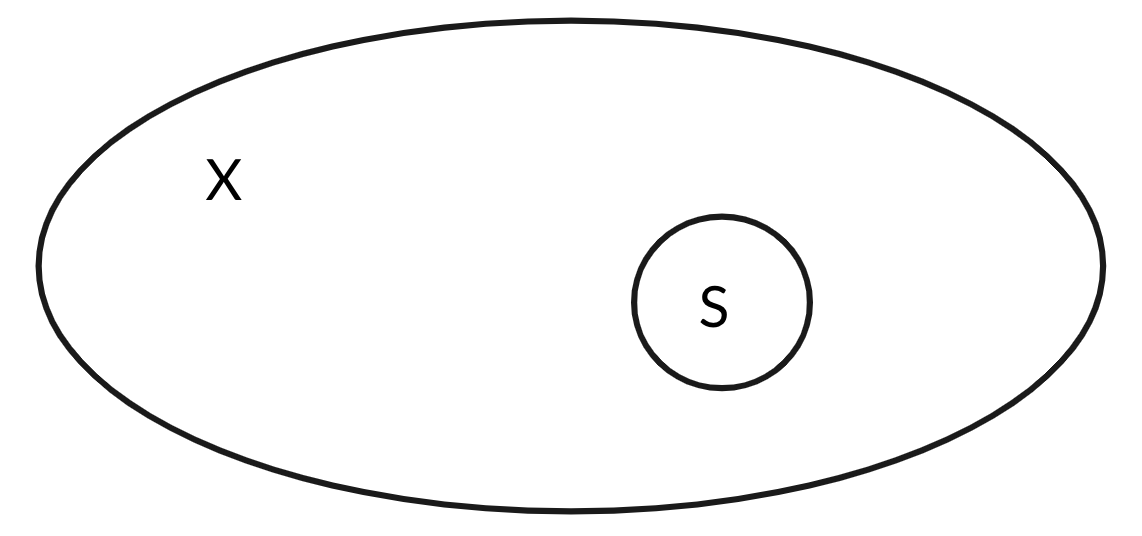
\includegraphics[origin=c,width=12cm]{../figures/independent-support.png}}
\caption{Visual Representation of an Independent Support}
\label{fig:ind_support}
\end{figure}

The primary target domain for UniGen is \textit{Constrained Random Verification} or CRV. In the domain of CRV, $|S|$ is typically significantly smaller than $|X|$, often by many orders of magnitude. UniGen exploits these observations by only applying variables in $S$ to the hash functions, which yields a significant reduction in the length of generated XOR clauses. Therefore, UniGen indeed scales to formulas with hundreds of thousands of variables, and even millions of clauses, but \textit{only} when $|S|$ remains small, typically $|S| < 100$. In the UniGen benchmarks, UniGen generated samples for over 200 different formulas. The largest of these, \texttt{demo3\_new}, had $865,935$ variables and $3,509,158$ clauses, but $|S|$ was only $45$. Similarly, the largest value of $|S|$ in the benchmarks was $78$ in \texttt{diagStencil\_new}, with $94,607$ variables and $2,838,579$ clauses. \cite{chakraborty_parallel_2015}

How does $|S|$ grow in the formulas generated by SweetPea? SweetPea currently selects all variables that directly represent level values for each factor in each trial as the independent support. For example, in the encoding shown in Table \ref{tab:encoding_diagram}, all 72 variables would be included in the independent support. However, the independent support does not include variables used to encode additional constraints or intermediate variables introduced during Tseitin encoding. While this set does not grow factorially, it still quickly grows into the hundreds and thousands, as shown in Table \ref{tab:benchmark_experiments_support}. While this independent support is certainly not minimal, we will see that even an optimal selection for the independent support could not guarantee $|S| < 100$.

\begin{table}[b]
  \centering
  \caption{Independent Support Size for Benchmark Experiments}
\begin{tabular}{|c|c|}
\hline
\multicolumn{1}{|l|}{Experiment Name}  & $|S|$   \\ \hline
stroop-2                               & 24      \\ \hline
stroop-3                               & 72      \\ \hline
stroop-4                               & 160     \\ \hline
stroop-5                               & 300     \\ \hline
stroop-congruency-balanced             & 270     \\ \hline
stroop-response                        & 526     \\ \hline
padmala-pessoa                         & 1,303   \\ \hline
task-switching                         & 636     \\ \hline
task-switching-2                       & 2,770   \\ \hline
% task-switching-cue-switching           & 24,594  \\ \hline
\end{tabular}
\label{tab:benchmark_experiments_support}%
\end{table}



There are a few simple improvements that could be made to the independent support computation today. Rather than including the variables for \textit{all} factors and levels in the independent support, it could exclude variables for derived factors whose levels are constrained by other factors. Additionally, a more efficient SAT encoding could be used based on combinations of variables rather than representing all levels as individual variables. (Although this would increase the complexity of encoding constraints.) Both of these would reduce $|S|$ by a degree, allowing UniGen to be useful for slightly larger formulas.

For any formula $F$ with independent support $S$, there are, by definition, exactly $2^{|S|}$ distinct assignments to $F$. Therefore, there can be no more than $2^{|S|}$ satisfying assignments, or solutions, to $F$. (In practice, the number of solutions will be much less, as not \textit{all} possible assignments will satisfy the formula.) Assuming an upper bound of $100$ for $|S|$, a perfectly efficient SAT encoding, and a minimal independent support, UniGen could only sample solutions to formulas with at most $2^{100}$ solutions. As seen in Table \ref{tab:benchmark_experiments}, SweetPea designs regularly exceed this threshold. Therefore, UniGen alone is insufficient for generating solutions, regardless of any potential improvements to the SAT encoding or the independent support computation.

\subsection{Benchmarks}

This shortcoming is proved out in practice. UniGen fails to count or sample from formulas where $|S| > 100$. Table \ref{tab:benchmark_experiments_unigen} denotes the time required for UniGen to generate 10 samples for each experiment. An estimate for $|R_F|$ is provided manually based on the factorial of the sequence length. Nearly all of them fail to complete in the allotted time (10 hours).

% Time to sample with 10 samples
% python -m timeit "__import__('os').system('unigen --verbosity=0 --kappa=0.638 --pivotUniGen=27 --maxLoopTime=3000 --maxTotalTime=36000 --pivotAC=60 --gaussuntil=400 --samples=10 --startIteration=13 stroop-3.cnf stroop3-unigen.out')"
% python -m timeit "__import__('os').system('unigen --verbosity=0 --kappa=0.638 --pivotUniGen=27 --maxLoopTime=3000 --maxTotalTime=36000 --pivotAC=60 --gaussuntil=400 --samples=10 --startIteration=38 stroop-4.cnf stroop4-unigen.out')"

\begin{table}[b]
  \centering
  \caption{Time to Generate 10 Samples with UniGen}
\begin{tabular}{|c|c|c|c|c|}
\hline
\multicolumn{1}{|l|}{Experiment Name} & Time to Sample  \\ \hline
stroop-2                              & -               \\ \hline
stroop-3                              & 2.18s           \\ \hline
stroop-4                              & Timed Out       \\ \hline
stroop-5                              & Timed Out       \\ \hline
stroop-congruency-balanced            & Timed Out       \\ \hline
stroop-response                       & Timed Out       \\ \hline
padmala-pessoa                        & Timed Out       \\ \hline
task-switching                        & Timed Out       \\ \hline
task-switching-2                      & Timed Out       \\ \hline
\end{tabular}
\label{tab:benchmark_experiments_unigen}
\end{table}


\section{Other Benchmarks}

As mentioned at the beginning of this chapter, we tested several other SAT samplers. This section presents the results of testing multiple SAT solving and sampling tools, as well as additional information on the implementation strategy of each tool. All sampling benchmarks were configured to generate ten samples at a time

\subsection{CryptoMiniSat}

CryptoMiniSat \cite{DBLP:conf/sat/SoosNC09} is a SAT solver. It is used internally by UniGen, as well as directly by SweePea to generate non-uniformly distributed trial sequences. SweetPea does non-uniform sampling by simply solving for any solution, then constraining the original formula to disallow that particular solution from being produced a second time. Due to the difficulty encountered while attempting to use SAT samplers, it has proven quite valuable to provide researchers with this ability to quickly generate some number of trial sequences conforming to their design, even though their distribution may be non-uniform. Sacrificing this guarantee allows them to quickly determine whether or not a particular design is even viable before investing additional resources. Lastly, in addition to logical \texttt{AND}, \texttt{OR}, and \texttt{NOT} clauses, CryptoMiniSat also natively supports \texttt{XOR} clauses, although SweetPea has not yet put these to use. (This is an opportunity for improvement.) Table \ref{tab:benchmark_experiments_cmsat} denotes the time required for CryptoMiniSat to compute a single solution to the SAT formula for each experiment.

% python -m timeit "__import__('os').system('cryptominisat5 padmala-pessoa.cnf > /dev/null')"

\begin{table}[b]
  \centering
  \caption{Time to Solve for 1 Solution with CryptoMiniSat}
\begin{tabular}{|c|c|c|c|c|}
\hline
\multicolumn{1}{|l|}{Experiment Name} & Time to Solve (ms)  \\ \hline
stroop-2                              & 4.9                 \\ \hline
stroop-3                              & 9.1                 \\ \hline
stroop-4                              & 18.9                \\ \hline
stroop-5                              & 64.4                \\ \hline
stroop-congruency-balanced            & 23.9                \\ \hline
stroop-response                       & 232                 \\ \hline
padmala-pessoa                        & 3,380               \\ \hline
task-switching                        & 140                 \\ \hline
task-switching-2                      & 200,000             \\ \hline
\end{tabular}
\label{tab:benchmark_experiments_cmsat}
\end{table}

The most complicated design for which SweetPea was able to construct a CNF encoding (\texttt{task-switching-2}) took the longest, at 200 seconds. CryptoMiniSat solved all other experiments in less than a second. Since this tool only generates a single solution, the practical time consideration is of minor importance here.


\subsection{KUS}

KUS \cite{SGRM18} is another SAT sampler developed by some of the same team behind UniGen. However, it approaches the problem quite differently. Rather than using hash functions to partition the solution space, KUS requires a compiled deterministic decomposable negation normal form (d-DNNF) of a formula. There are known polynomial-time techniques for many operations on the d-DNNF representation of a Boolean formula, including model counting. KUS takes advantage of these techniques to sample solutions using this form uniformly. This technique offloads much of the complexity to the d-DNNF compiler, rather than the sampling phase. KUS, while able to sample quickly, is not used in SweetPea due to scaling problems in compiling the d-DNNF form. Though the number of variables and clauses in the CNF for a formula is typically modest, compiling the equivalent d-DNNF has proven intractable. Table \ref{tab:benchmark_experiments_d4} denotes the time required to compile the CNF for each experiment to d-DNNF using the \texttt{d4} compiler, as well as the resulting d-DNNF file size,  compared to the original CNF file.

% TIme to compile d-DNNF
% Size of a d-DNNF file vs. original CNF, % increase in file size?

% Time to sample with 10 samples.
% time timelimit -T 36000 -t 36000 /home/drautb/GitHub/meelgroup/KUS/d4 cnfs/stroop-congruency-balanced.cnf -out=d-DNNFs/stroop-congruency-balanced.dnnf

% ➜  benchmark-experiments git:(master) ✗ time timelimit -T 36000 -t 36000 /home/drautb/GitHub/meelgroup/KUS/d4 cnfs/task-switching-2.cnf -out=d-DNNFs/task-switching-2.dnnf
% c WARNING: for repeatability, setting FPU to use double precision
% c Problem Statistics:
% c
% c Benchmark Information
% c Number of variables: 742832
% c Number of clauses: 2043674
% c Number of literals: 5958852
% c Parse time: 0.39
% c
% ===============================================================================
% INDETERMINATE
% timelimit -T 36000 -t 36000 /home/drautb/GitHub/meelgroup/KUS/d4    18709.93s user 7.88s system 99% cpu 5:12:08.05 total

\begin{table}[b]
  \centering
  \caption{d-DNNF Compilation for Sampling with KUS}
\begin{tabular}{|c|c|c|c|c|}
\hline
\multicolumn{1}{|l|}{Experiment Name} & Time            & d-DNNF               & CNF            & \% Growth   \\ \hline
stroop-2                              & 14.4ms          & 9.7K                 & 24K            & -60\%       \\ \hline
stroop-3                              & 1.99s           & 6.3M                 & 151K           & 4,072\%     \\ \hline
stroop-4                              & Timed Out       & -                    & 303K           & -           \\ \hline
stroop-5                              & Timed Out       & -                    & 881K           & -           \\ \hline
stroop-congruency-balanced            & 48.6m           & 7.3G                 & 447K           & 1,633,009\% \\ \hline
stroop-response                       & Timed Out       & -                    & 1.5M           & -           \\ \hline
padmala-pessoa                        & OOM             & -                    & 13M            & -           \\ \hline
task-switching                        & Timed Out       & -                    & 1.2M           & -           \\ \hline
task-switching-2                      & "Indeterminate" & -                    & 92M            & -           \\ \hline % (5.2 hrs)
\end{tabular}
\label{tab:benchmark_experiments_d4}
\end{table}

For the experiments for which the d-DNNF compiler completed, Table \ref{tab:benchmark_experiments_kus} denotes the time required to sample solutions using KUS.

% ➜  benchmark-experiments git:(master) ✗ time timelimit -T 36000 -t 36000 python /home/drautb/GitHub/meelgroup/KUS/KUS.py --dDNNF ~/Desktop/stroop-congruency-balanced.dnnf --samples 10 --outputfile d-DNNFs/stroop-congruency-balanced-kus-10-samples.out
% timelimit -T 36000 -t 36000 python /home/drautb/GitHub/meelgroup/KUS/KUS.py    11.39s user 11.16s system 5% cpu 7:05.45 total

\begin{table}[b]
  \centering
  \caption{Time to Generate 10 Samples with KUS}
\begin{tabular}{|c|c|c|c|c|}
\hline
\multicolumn{1}{|l|}{Experiment Name} & Time        \\ \hline
stroop-2                              & 92.7 ms     \\ \hline
stroop-3                              & 2.35 s      \\ \hline
stroop-4                              & -           \\ \hline
stroop-5                              & -           \\ \hline
stroop-congruency-balanced            & OOM         \\ \hline  % 7mins 5s
stroop-response                       & -           \\ \hline
padmala-pessoa                        & -           \\ \hline
task-switching                        & -           \\ \hline
task-switching-2                      & -           \\ \hline
task-switching-cue-switching          & -           \\ \hline
\end{tabular}
\label{tab:benchmark_experiments_kus}%
\end{table}

As expected, sampling occurs quickly once a reasonably-sized d-DNNF file has been obtained. However, the combinatorial nature of experimental designs makes the cost of compiling and interpreting the d-DNNF prohibitive.


\subsection{Spur}

Spur \cite{spur} is a more recent SAT sampler that employs reservoir sampling. In benchmarks, it performs better than UniGen in nearly all cases. However, it does require an exact model count (based on sharpSAT), while an approximation suffices for UniGen. SweetPea does not rely on Spur at present, as it did not exist at SweetPea's inception. However, we consider it here as it represents the latest research for SAT sampling. Table \ref{tab:benchmark_experiments_spur} denotes the time required to generate samples for each experiment using Spur, with results similar to other tools.

% Time to get a model count.

% Time to sample 10 samples

% ➜  benchmark-experiments git:(master) ✗ time timelimit -T 36000 -t 36000 ~/GitHub/ZaydH/spur/build/Release/spur -cnf cnfs/task-switching-2.cnf -s 10
% WARNING: No sample results file specified.
% Using default filename: "cnfs/samples_task-switching-2.txt"
% Performing Uniform Model Sampling...
% Input File:  cnfs/task-switching-2.cnf
% Output File: cnfs/samples_task-switching-2.txt

% Preprocessing ... DONE
% variables (all/used/free):      742832/742832/0
% independent support size:       2770
% clauses (all/long/binary/unit): 3672632/3133493/384324/154815
% terminate called after throwing an instance of 'std::bad_alloc'
%   what():  std::bad_alloc
% timelimit -T 36000 -t 36000 ~/GitHub/ZaydH/spur/build/Release/spur -cnf  -s 1  71.16s user 6.95s system 62% cpu 2:04.49 total


\begin{table}[b]
  \centering
  \caption{Time to Generate 10 Samples with Spur}
\begin{tabular}{|c|c|c|c|c|}
\hline
\multicolumn{1}{|l|}{Experiment Name} & Time to Sample                \\ \hline
stroop-2                              & 21.9 ms                       \\ \hline
stroop-3                              & 3.72 s                        \\ \hline
stroop-4                              & Timed Out                     \\ \hline
stroop-5                              & Timed Out                     \\ \hline
stroop-congruency-balanced            & OOM                           \\ \hline  % 5hrs 5mins
stroop-response                       & Error                         \\ \hline  % 7hrs 52mins
padmala-pessoa                        & Timed Out                     \\ \hline  % 10hrs
task-switching                        & Timed Out                     \\ \hline  % 10hrs
task-switching-2                      & Error                         \\ \hline  % 2hrs 5mins
task-switching-cue-switching          & -                             \\ \hline  % Don't have CNF
\end{tabular}
\label{tab:benchmark_experiments_spur}%
\end{table}

As with other Samplers, Spur can successfully generate samples for only the smallest designs.


\section{Sample Distribution}

As has been mentioned several times, there must be a one-to-one relationship between unique trial sequences and solutions to the SAT formula in order for uniformity guarantees to carry over from the SAT sampler results back to the original problem space. In this section, we will examine the distribution of the trial sequences produced by UniGen, KUS, and Spur, providing empirical evidence that the resulting trial sequences follow a uniform distribution.

We sampled 10,000 trial sequences for the Stroop-3 experiment using UniGen, KUS, and Spur. The resulting samples follow a uniform distribution; each sample only occurred once in the vast majority of cases.

\subsection{UniGen}

UniGen sampled 10,010 trial sequences, 9,965 of which were unique. Numbering each unique trial sequence in the order that it appeared and generating a histogram gives a visual confirmation that the sequences are approximately uniform. UniGen generated 333 sequences twice and only generated six three times. It generated no sequences more than three times. Figure \ref{fig:unigen_samples} shows the sequence distribution.

\begin{figure}[b]
\centering
\centerline{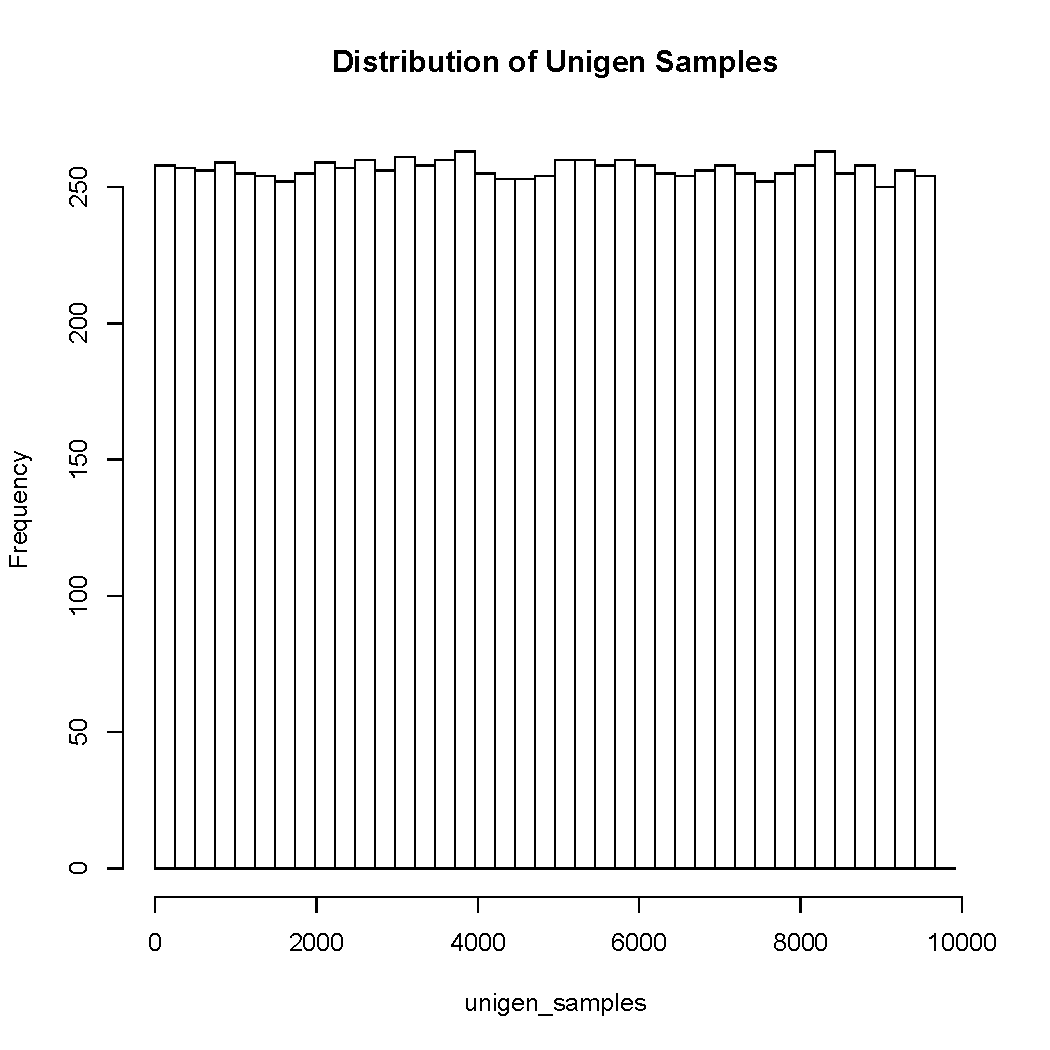
\includegraphics[origin=c,width=12cm]{../figures/unigen-samples.pdf}}
\caption{Distribution of Sequences Sampled by UniGen}
\label{fig:unigen_samples}
\end{figure}


\subsection{KUS}

% time python /home/drautb/GitHub/meelgroup/KUS/KUS.py --dDNNF d-DNNFs/stroop-3.dnnf --samples 10000 --outputfile d-DNNFs/stroop-3-kus-10000-samples.out
% ('Time taken to parse the nnf text:', 1.0481359958648682)
% ('Time taken for Model Counting:', 1.0421910285949707)
% ('Model Count:', 112409849997702614628L)
% ('Time taken by sampling:', 16.441092014312744)
% ('Samples saved to', 'd-DNNFs/stroop-3-kus-10000-samples.out')
% python /home/drautb/GitHub/meelgroup/KUS/KUS.py --dDNNF d-DNNFs/stroop-3.dnnf  25.76s user 0.59s system 102% cpu 25.828 total

KUS sampled 10,000 trials sequences, all of which were unique. Figure \ref{fig:kus_samples} shows the sequence distribution.

\begin{figure}[t]
\centering
\centerline{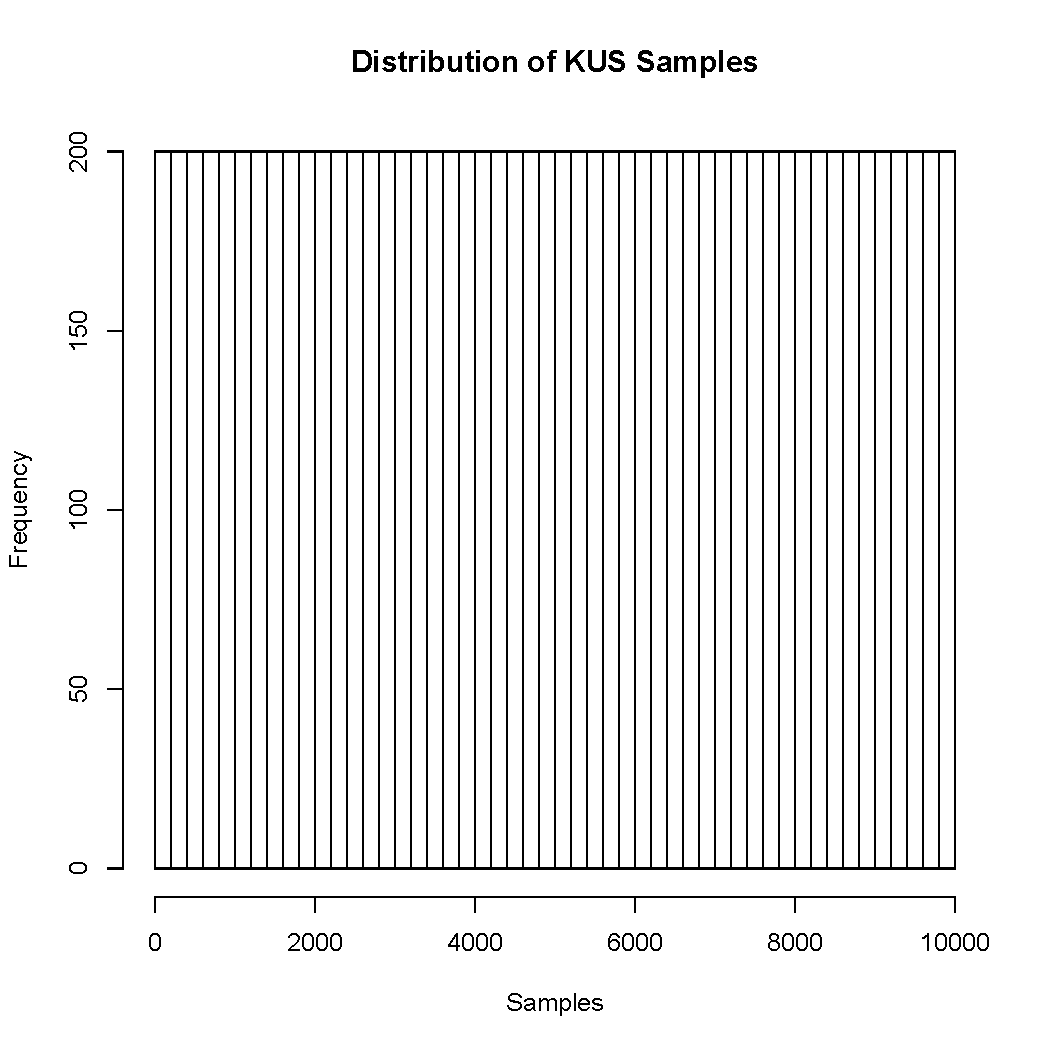
\includegraphics[origin=c,width=12cm]{../figures/kus-samples.pdf}}
\caption{Distribution of Sequences Sampled by KUS}
\label{fig:kus_samples}
\end{figure}


\subsection{Spur}

% time /home/drautb/GitHub/ZaydH/spur/build/Release/spur -q -s 10000 -cnf stroop-3.cnf -out stroop-3-spur-10000-samples.out
% /home/drautb/GitHub/ZaydH/spur/build/Release/spur -q -s 10000 -cnf  -out   30.97s user 0.23s system 99% cpu 31.250 total

Spur sampled 10,000 trial sequences, 9,664 of which were unique. It generated three hundred thirty-two sequences twice and two sequences three times. It generated no sequences more than three times. Figure \ref{fig:spur_samples} shows the sequence distribution.

\begin{figure}[t]
\centering
\centerline{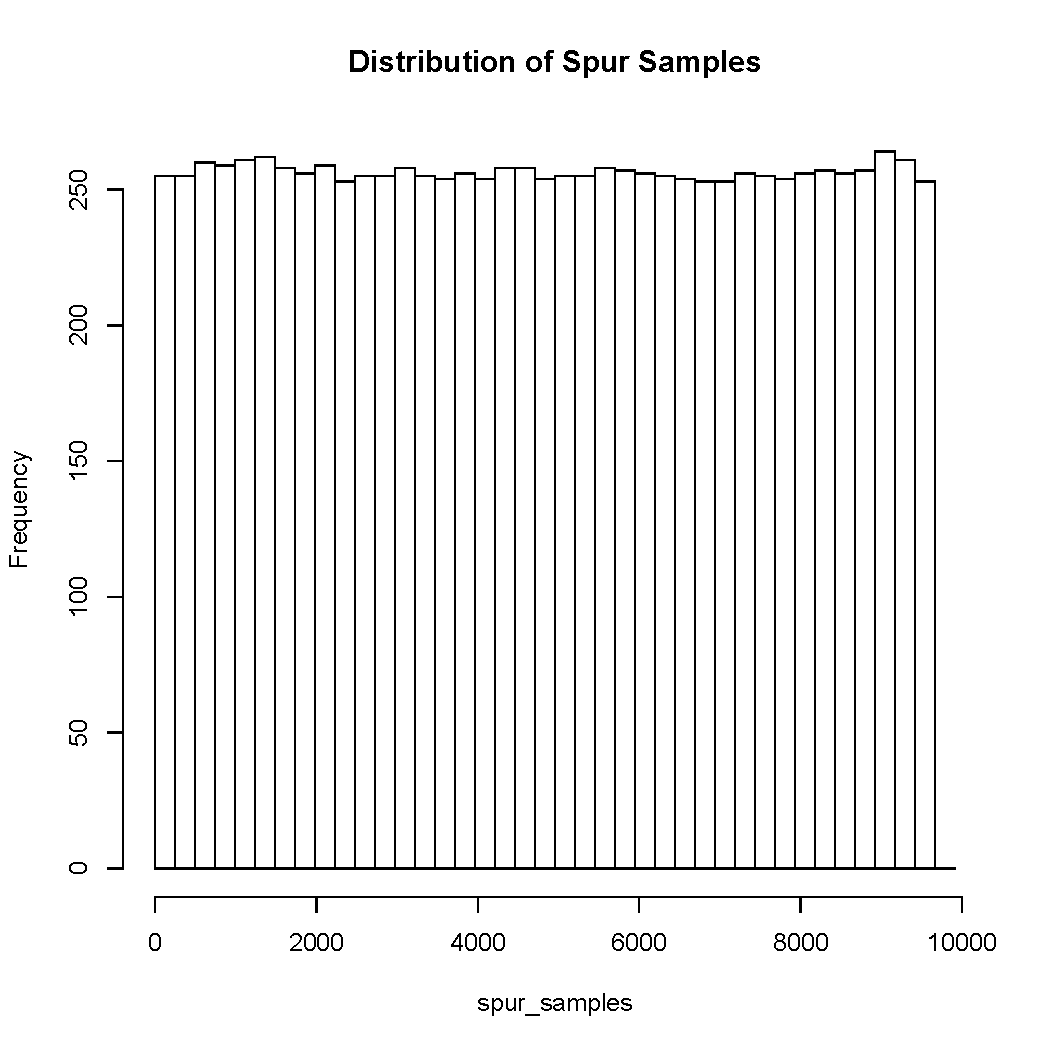
\includegraphics[origin=c,width=12cm]{../figures/spur-samples.pdf}}
\caption{Distribution of Sequences Sampled by Spur}
\label{fig:spur_samples}
\end{figure}

\subsection{CryptoMiniSat}

In contrast to the previous tests, when a SAT solver is used to generate individual samples incrementally by adding negated solutions to the prior formula, the same samples are generated each time. We used CryptoMiniSat to generate 10,000 samples as well, in groups of 100. It generated precisely the same set of 100 samples each time.


Of all the Samplers tested, KUS produced the most uniformly distributed samples.

\bigbreak
\bigbreak

\section{Summary}

We had hoped that UniGen would be able to generate uniformly-distributed solutions for experimental designs, in particular because the volume of variables and clauses in our generated CNF files fell within the range of example benchmarks provided by the UniGen authors. However, we overlooked the role played by the magnitude of the independent support set. Because UniGen requires the size of the independent support set to be less than 100 variables, there is a limit to the number of solutions a formula may have in order for UniGen to be effective. For realistic experimental designs, the number of solutions quickly outstrips this bound. Furthermore, none of the additional tested tools for sampling SAT formulae are capable of handling the scale of practical experimental designs. Although these experiments contain a reasonable number of variables and clauses, the

\newpage

\noindent factorial explosion in the solution space, as well as the magnitude of the independent support set, proved too large.
